\chapter{Głębokie sieci neuronowe}
\thispagestyle{chapterBeginStyle}

\section{Opis architektury}

Do przewidywania pozycji wyjściowych agenta \texttt{EGO} można wykorzystać głębokie sieci neuronowe. Rozważane w tej pracy sieci neuronowe składają się ze szkieletu odpowiadającego za przetwarzanie rasteryzowanych scen (głębokie sieci konwolucyjne) oraz z części składającej się z gęstych warstw odpowiadającej za dalsze przetworzenie wyjść z sieci szkieletowej na przewidywane pozycje wyjściowe agenta \texttt{EGO}.

\begin{figure}[htbp]
    \centering
    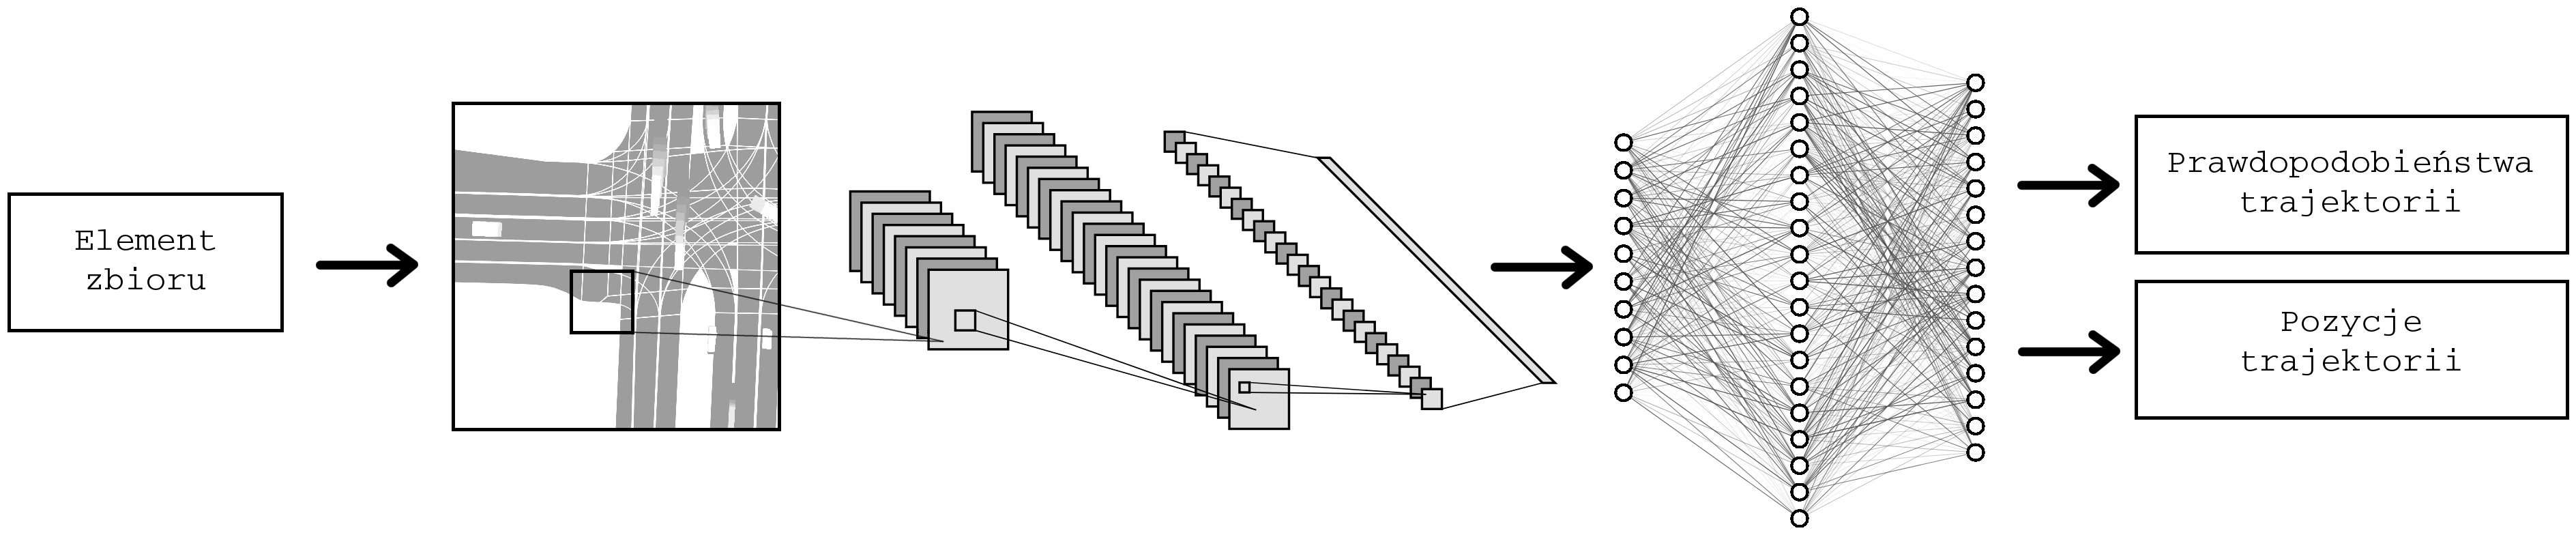
\includegraphics[width=\linewidth]{nn_schema.png}
    \caption{Wizualizacja architektury sieci neuronowej}
\end{figure}

\noindent
Proces predykcji opisanej sieci neuronowej przebiega w następujący sposób:
\begin{itemize}
    \setlength{\itemsep}{1pt}
    \setlength{\parskip}{0pt}
    \setlength{\parsep}{0pt}
    \item Ustalony zostaje indeks próbki (próbka to element zbioru).
    \item Wczytane zostają wszystkie dane dotyczące próbki (agenci, pasy, światła itd.)
    \item Następuje rasteryzacja próbki (stworzenie podglądu sceny)
    \item Otrzymany obraz jest przetwarzany przez szkielet sieci (część składająca się z warstw konwolucyjnych).
    \item Wektor cech podawany jest na wejście gęsto połączonej sieci neuronowej. Sieć ta zwraca wektor posiadający prawdopodobieństwa trajektorii i pozycje przewidywanych trajektorii.
\end{itemize}

\noindent
Szkielet sieci domyślnie przyjmuje obrazy o wymiarach $(3, H, W)$, lecz rasteryzator \texttt{SemBoxRasterizer} zwraca obrazy o wymiarach $(25, H, W)$, gdzie kanały posiadają następujące informacje:

\begin{itemize}
    \setlength{\itemsep}{1pt}
    \setlength{\parskip}{0pt}
    \setlength{\parsep}{0pt}
    \item 0-11 zawierają zaznaczone wejściowe pozycje agenta \texttt{EGO} w chwilach \mbox{$[t, t-0.1, ... , t-1.0]$}
    \item 11-22 zawierają zaznaczone wejściowe pozycje agentów innych niż \texttt{EGO} w chwilach \mbox{$[t, t-0.1, ... , t-1.0]$}
    \item 23-25 zawierają rasteryzowaną scenę w formacie RGB (wszystkie informacje agenci, pasy, światła itd.)
\end{itemize}

Z tego powodu wymagana jest modyfikacja pierwszej warstwy konwolucyjnej w domyślnych sieciach szkieletowych. Pierwsza warstwa konwolucyjna jest usuwana i zastępowana jest warstwą o tych samych argumentach (padding, stride itp), z wyjątkiem liczby kanałów wejściowych, która zamieniana jest z 3 na 25. Trzeba zaznaczyć, że wykonywane jest to tylko przy korzystaniu z rasteryzatora \texttt{SemBoxRasterizer}, w przypadku rasteryzatora \texttt{CenterLines} pierwsza warstwa konwolucyjna nie jest modyfikowana, gdyż rasteryzator ten zwraca obraz z trzema kanałami.

\newpage

\subsection{Szczegółowy opis warstw sieci}

\begin{itemize}
    \setlength{\itemsep}{1pt}
    \setlength{\parskip}{0pt}
    \setlength{\parsep}{0pt}
    \item Szkielet sieci przyjmuje obraz o wymiarach $(3, H, W)$ lub $(25, H, W)$
    \item Szkielet sieci zwraca wektor długości \texttt{backbone\_out\_features} w zależności od użytego typu sieci:
        \begin{itemize}
            \setlength{\itemsep}{1pt}
            \setlength{\parskip}{0pt}
            \setlength{\parsep}{0pt}
            \item \texttt{ResNet-18}: 512
            \item \texttt{ResNet-34}: 512
            \item \texttt{ResNet-50}: 2048
            \item \texttt{EfficientNet-B3}: 1536
            \item \texttt{EfficientNet-B5}: 2048
            \item \texttt{EfficientNet-B6}: 2304
            \item \texttt{MixNet-M}: 1536
            \item \texttt{MixNet-L}: 1536
        \end{itemize}
    \item Warstwa głęboko połączona przyjmuje wektor długości \texttt{backbone\_out\_features}, zwraca wektor długości 4096. Nakładana jest funkcja aktywacji \texttt{ReLU}.
    \item Warstwa głęboko połączona przyjmuje wektor długości 4096, zwraca wektor długości 303 odpowiadający elementom tensora zawierającego 3 trajektorie (w 2 wymiarach: x oraz y) i 3 prawdopodobieństwa trajektorii. Stąd $303 = 3*(50 * 2 + 1)$
\end{itemize}

\section{Szkielet sieci neuronowej}

\subsection{Ogólne porównanie}

\begin{center}
\begin{tabular}{ |c|c|c|c|c| } 
\hline
Nazwa sieci & Data opublikowania & Liczba parametrów & ImageNet błąd Top1 & ImageNet błąd Top5\\
\hline
ResNet-18 & 10.12.2015r. & 11.2 mln & 30.2 & 10.9\\
\hline
ResNet-34 & 10.12.2015r. & 21.3 mln & 26.7 & 8.6\\
\hline
ResNet-50 & 10.12.2015r. & 23.6 mln & 23.9 & 7.1\\
\hline
EfficientNet-B3 & 28.05.2019r. & 12.0 mln & 18.4 & 4.3\\
\hline
EfficientNet-B5 & 28.05.2019r. & 30.0 mln & 16.4 & 3.3\\
\hline
EfficientNet-B6 & 28.05.2019r. & 43.0 mln & 16.0 & 3.2\\
\hline
MixNet-M & 22.07.2019r. & 5.0 mln & 23.0 & 6.7\\
\hline
MixNet-L & 22.07.2019r. & 7.3 mln & 21.1 & 5.8\\
\hline
\end{tabular}
\end{center}

\subsection{\texttt{ResNet}}
Głębokie sieci neuronowe bywają trudne w trenowaniu, często wynika to z efektu zanikających oraz eksplodujących gradientów. Architektura \texttt{ResNet} \cite{1512.03385} była jednym z pierwszych udanych rozwiązań tego problemu w odniesieniu do problemów wizji z użyciem sieci \texttt{CNN} (sieci konwolucyjnych). Pozwoliło to na zwiększenie głębokości sieci neuronowych, co przyczyniło się do polepszenia skuteczności sieci \texttt{CNN}. Obecnie istnieje wiele lepszych architektur sieci  \texttt{CNN} pod względem wyników na zbiorach porównawczych takich jak np. \texttt{ImageNet} \cite{deng2009imagenet}, mimo to sieci \texttt{ResNet} dalej są wykorzystywane ze względu na bardzo dobry kompromis pomiędzy skomplikowaniem architektury, a skutecznością.

\newpage

\subsection{\texttt{EfficientNet}}
Bardzo często architektury sieci neuronowych są projektowane z myślą o ograniczeniach zasobów obliczeniowych (szybkość predykcji oraz zapotrzebowanie na pamięć \texttt{RAM}). Sieci o architekturze \texttt{EfficientNet} \cite{1905.11946} zostały zaprojektowane z myślą o jak najlepszym wykorzystaniu dostępnych zasobów. Wykorzystują obserwację dotyczącą skalowania sieci, która pozwala na efektywne wykorzystanie zasobów. Powiększanie sieci w celu uzyskania lepszej jakości predykcji odbywa się nie tylko względem głębokości sieci (dodawanie kolejnych warstw konwolucyjnych). Autorzy architektury \texttt{EfficientNet} pokazali technikę, która pozwala na skalowanie głębokości, szerokości oraz rozdzielczości sieci w optymalny sposób, przy ograniczeniach na liczbę operacji zmiennoprzecinkowych na sekundę oraz używanej pamięci \texttt{RAM}. Otrzymane architektury zostały znalezione za pomocą przeszukiwania przestrzeni sieci neuronowych techniką \texttt{NAS} (ang. neural architecture search).

\subsection{\texttt{MixNet}}
Sieci konwolucyjne zazwyczaj wykorzystują konwolucję \texttt{Depthwise}, jest to typ konwolucji, której jądro obliczane jest z wykorzystaniem wszystkich kanałów jednocześnie (w odpowiednich obszarach każdego z kanałów). Sieci architektury \texttt{MixNet} \cite{1907.09595} zostały zaprojektowane z zamiarem wykorzystania wielu rozmiarów jądra konwolucji bez zbędnego zwiększania liczby parametrów sieci. Zaproponowany został w tym celu rodzaj konwolucji \texttt{MixConv}, który wykorzystuje jednocześnie wiele rozmiarów jądra w jednej konwolucji. Konwolucja \texttt{MixConv} została dodana jako jedna z opcji przy przeszukiwaniu przestrzeni sieci neuronowych techniką \texttt{NAS}. Otrzymane w wyniku przeszukiwania architektury należą do rodziny \texttt{MixNet} i wykorzystują konwolucje \texttt{MixConv}.

\section{Pretrenowanie sieci}
Opisane powyżej architektury szkieletów głębokich sieci konwolucyjnych są bardzo czasochłonne w trenowaniu. Z tego względu przy wykorzystaniu tych szkieletów do zadań wizji, wykorzystuje się tzw. pretrenowanie (ang. pre-training) \cite{1901.09960}. Jest to proces polegający na trenowaniu sieci na podobnym zbiorze do zbioru docelowego (tego, który wykorzystany zostanie do nauczenia konkretnego zadania). Najczęściej pretrenowanie odbywa się na zbiorze \texttt{ImageNet}, sieć trenowana jest na zadaniu klasyfikacji jednej z tysiąca klas obiektów obecnych w zbiorze. Na końcu pretrenowania usuwa się ostatnią warstwę sieci (głęboko połączona warstwa odpowiedzialna za klasyfikację). Dzięki temu procesowi uzyskana sieć potrafi rozróżniać kształty, kolory oraz podstawowe obiekty. Następnie wystarczy dokończyć proces trenowania na zadaniu, które rozpatrujemy. Proces pretrenowania ma za zadanie oszczędzić czas potrzebny na wyuczenie sieci podstawowych informacji o strukturze danych wejściowych (w tym wypadku obrazy). W tej pracy każdy wykorzystany szkielet został poddany procesowi pretrenowania, parametry tych sieci są pobierane z biblioteki \texttt{torchvision}. Parametrami tymi inicjalizuje się odpowiednie architektury sieci neuronowych.